\section{Software Monoliths}\label{section:background:software-monolith}

A monolithic architecture is characterized that there is only one single codebase. Many developers, no matter from which team are working on the same application. This approach to development was the standard for a very long time and is well supported by various modern development tools. By just having one application the developers have a complete overview over the complete application. A single database with one schema is mostly used for this software development approach. A prototypical architecture for a monolithical application is shown in figure \ref{fig:background:monolith:monolith-sketch}.

\ifshowImages
\begin{figure}[H]
    \centering
    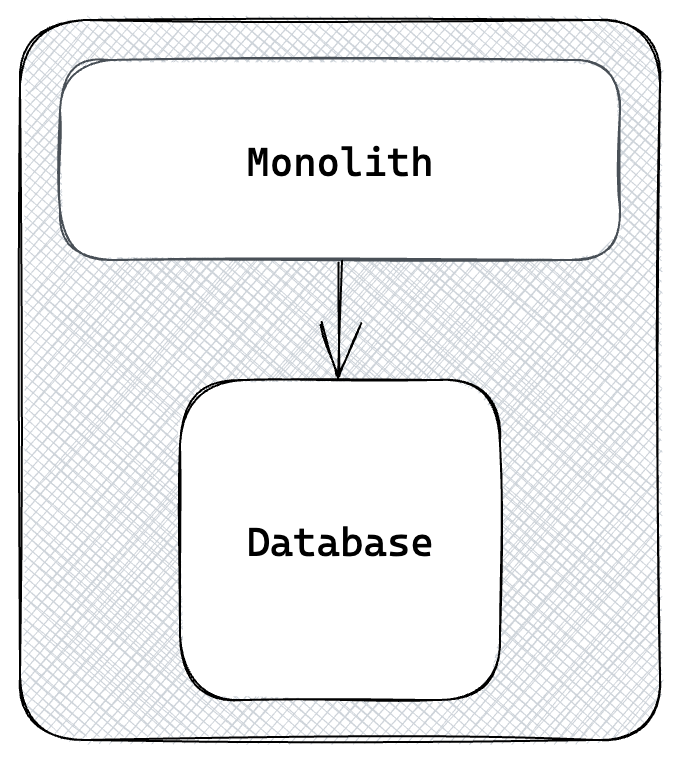
\includegraphics[width=0.3\linewidth]{images/background/monolith/monolith-sketch.png}
    \caption{The typical architecture of a monolithical application. (Adapted from \cite[12]{book:2019:newman:background:monolith:monolith-to-microservices})}\label{fig:background:monolith:monolith-sketch}
\end{figure}
\fi

\bigskip

\noindent With a monolith it is easier to apply drastic changes to the complete codebase. Modern IDE support refactoring properties for example over the complete project. Therefore it is relatively easy to apply changes to every layer of the application, even the database schema. All parts of the project can be tested directly by running the application and the related database. And the complete application can be built and deployed in one step. And it is easy to scale, as multiple instances can be run behind a load balancer. \cite[4]{book:2018:richardson:background:bff:microservices-patterns}

\bigskip

\noindent If a monolith starts to grow in size, it is important to have a good software architecture. The code should be put in modules, which follow the rules of high cohesion and low coupling of code elements. The modularization just splits the code into multiple chunks, which are easier to understand, but the application is still just a single process. Modules can be developed separately, but the application has to be deployed as one unit. This requires coordination of various development teams. \cite[12-13]{book:2018:richardson:background:bff:microservices-patterns} \cite[12-13]{book:2019:newman:background:monolith:monolith-to-microservices} Such an architecture is shown in listing \ref{fig:background:monolith:module-monolith-sketch}.

\ifshowImages
\begin{figure}[H]
    \centering
    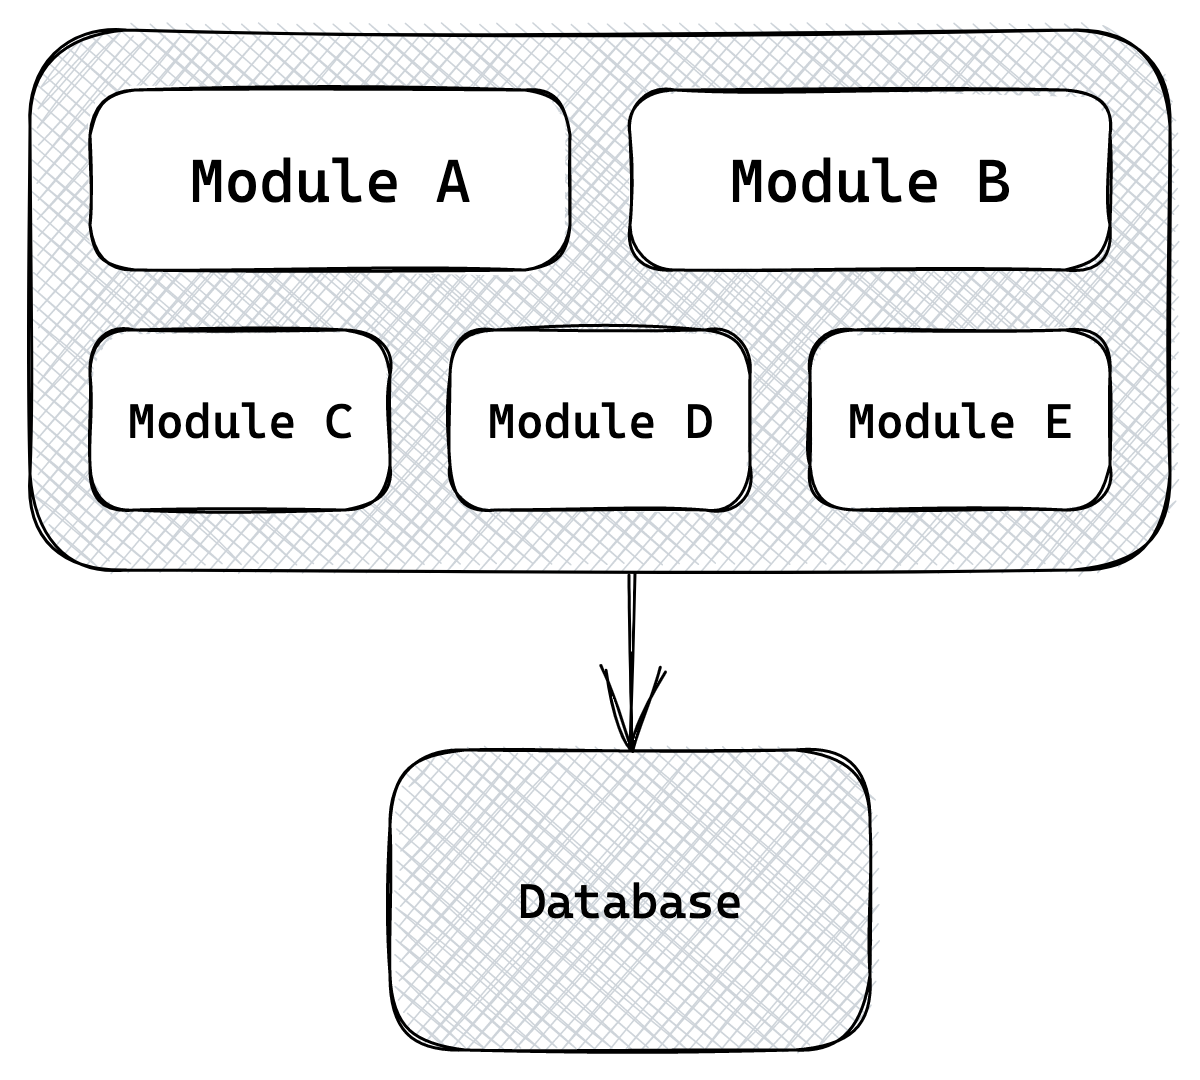
\includegraphics[width=0.4\linewidth]{images/background/monolith/modular-monolith-sketch.png}
    \caption{Structure of a modular monolith (Adapted from \cite[13]{book:2019:newman:background:monolith:monolith-to-microservices})}\label{fig:background:monolith:module-monolith-sketch}
\end{figure}
\fi

\noindent Modular monoliths provide an excellent choice for a lot of organizations. If there are well defined module boundaries, parallel working is possible quite easily. But a database lacks the possibility of decomposing the logic like on the code level. \cite[12-13]{book:2019:newman:background:monolith:monolith-to-microservices}

\subsection{Disadvantages}\label{subsection:background:software-monolith:disadvantages}

With a growing code base, monolithic architectures come with increased complexity. Each new feature adds another level of complexity, which leads to reduced developer performance. Developing a new feature might be a very long process, due to the existing entry hurdle. The sheer size of the code base makes it difficult to understand, because program comprehension is a very important factor for the maintenance of software. \cite{article:1995:mayrhauser:background:monoliths:program-comprehension-during-software-maintenance-and-evolution} Therefore, developers might create side effects when fixing a bug. The time for developing a new feature increases drastically and the internal architecture can become difficult to understand and maintain as well. \cite[4-6]{book:2018:richardson:background:bff:microservices-patterns}

\bigskip

\noindent Another problem is, that multiple teams might work on the same chunks of code. It might happen that two different developers need to make a change to code in a shared library. It might happen that a developer changes code inside a module, where he doesn't have enough knowledge about. The change might be also not coordinated with other software engineers. This might lead to unexpected behavior in the code of the other developer. The circumstance is also \textit{confused lines of ownership}, which are sources of failures for a software system. \cite[15]{book:2019:newman:background:monolith:monolith-to-microservices} \cite[7]{inproceedings:2011:bird:background:monoliths:dont-touch-my-code}

\bigskip

\noindent With a monolithic approach, the use of different technologies is not possible anymore. The technology stack is restricted to the entire life of the monolith. The introduction of a different programming language or a different framework is hardly possible and often leads to a complete rewrite of an application. \cite[6-7]{book:2018:richardson:background:bff:microservices-patterns} The problem with technology is that it always becomes deprecated and obsolete at one point in time. Applications based on such frameworks have to be migrated to a different programming language or framework. Simply rewriting the application in another framework is not simple, because every functionality of the application has to be understood.

\subsubsection{Monolithic Systems are not Legacy Systems}\label{subsection:background:software-monolith:not-legacy-systems}

Writing a monolithic application should not be synonymous with writing a legacy application. The term legacy should not be used with monolithic systems. \cite[15]{book:2019:newman:background:monolith:monolith-to-microservices} The monolithic architecture is a good starting point for a new applications. If some domains of the applications are not well understood and when drastic changes can happen to already implemented features. It is easier to understand the complete application and to make changes to the code. \cite[43]{book:2019:newman:background:monolith:monolith-to-microservices}
